%
% Capítulo 3
%
\chapter{Solução do Problema} \label{cap3}

\section{Modelo de Dados}\label{sec31}

% Modelo EA
\subsection{Modelo Entidade-Associação}

\begin{figure}
	\centering
	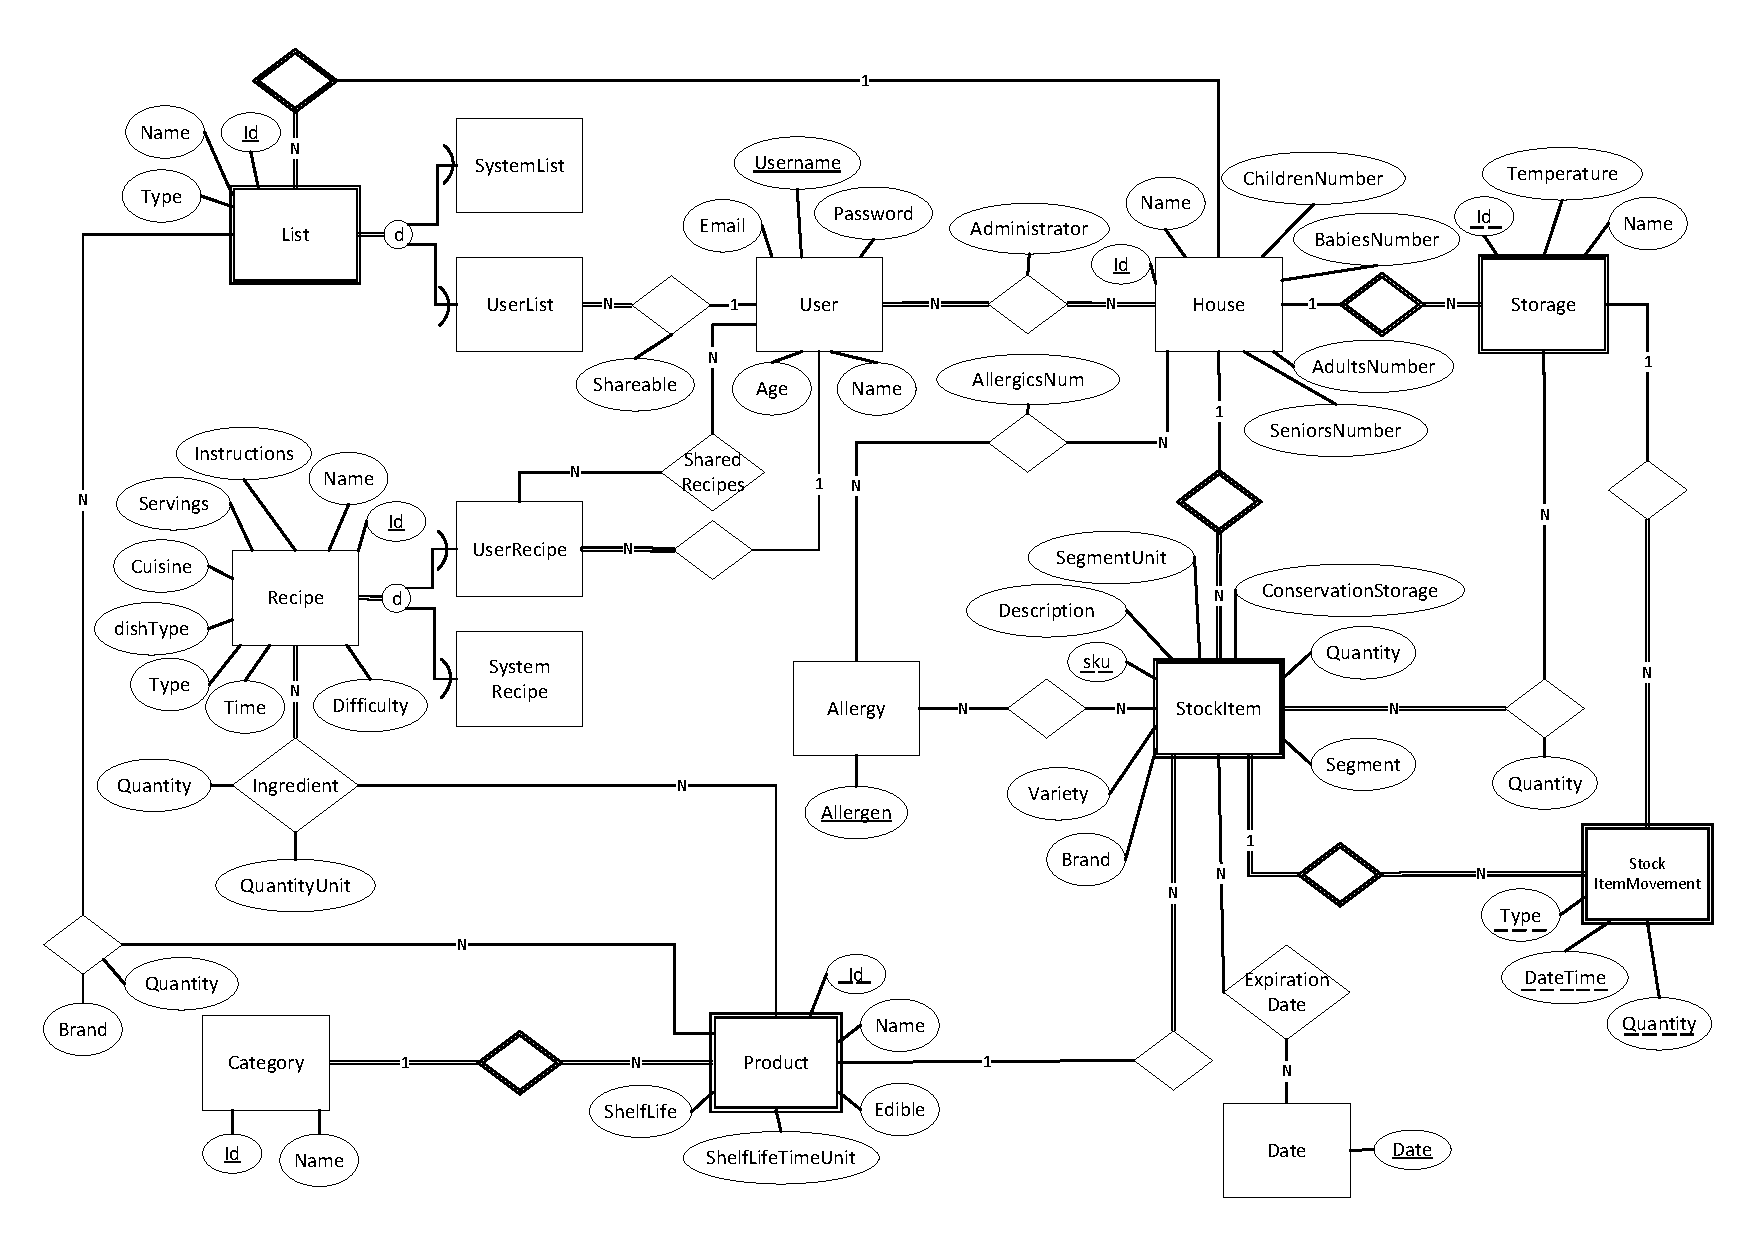
\includegraphics[width=20cm,height=16cm,scale=0.5]{./files/EA.pdf}
	\caption{Modelo Entidade-Associação}
	\label{modelo-ea}
\end{figure}

% Modelo Relacional
\subsection{Modelo Relacional}
{\parindent 0pt
	\begin{description}
		\item House(house\_id, house\_name, house\_babiesNumber, house\_childrenNumber, house\_adultsNumber, house\_seniorsNumber) \newline
		\acrshort{cp}: (house\_id) 
		
		\item User(user\_username, user\_email, user\_age, user\_name, user\_password) \newline
		\acrshort{cp}: (user\_username)  \newline
		\acrshort{occ}: (user\_email)
		
		\item Allergy(allergy\_allergen) \newline
		\acrshort{cp}: (allergy\_allergen) 
		
		\item Recipe(recipe\_id, recipe\_name, recipe\_instructions, recipe\_difficulty, recipe\_time, recipe\_servings, recipe\_cuisine, recipe\_dishType, recipe\_type) \newline
		\acrshort{cp}: (recipe\_id) 
		
		\item SystemRecipe(recipe\_id) \newline
		\acrshort{cp}: (recipe\_id) \newline
		\acrshort{ce}: \{(recipe\_id) ref Recipe\}
		
		\item UserRecipe(recipe\_id, user\_username) \newline
		\acrshort{cp}: (recipe\_id) \newline
		\acrshort{ce}: \{(recipe\_id) ref Recipe, (user\_username) ref User\}
		
		\item SharedRecipe(recipe\_id, user\_username) \newline
		\acrshort{cp}:(recipe\_id, user\_username) \newline
		\acrshort{ce}: \{(recipe\_id) ref Recipe, (user\_username) ref User\}
		
		\item List(house\_id, list\_id, list\_name, list\_type) \newline
		\acrshort{cp}: (house\_id, list\_id) \newline
		\acrshort{ce}: \{(house\_id) ref House\}
		
		\item SystemList(house\_id, list\_id)
		\newline
		\acrshort{cp}: (house\_id, list\_id) \newline
		\acrshort{ce}: \{(house\_id, list\_id) ref List\}
		
		\item UserList(house\_id, list\_id, user\_username, list\_shareable)
		\newline
		\acrshort{cp}: (house\_id, list\_id) \newline
		\acrshort{ce}: \{(house\_id, list\_id) ref List, (user\_username) ref User\}
		
		\item Category(category\_id, category\_name)
		\newline
		\acrshort{cp}: (category\_id) \newline
		\acrshort{occ}: (category\_name)
		
		\item Product(category\_id, product\_id, product\_name, product\_edible, product\_shelfLife, \newline product\_shelfLifeTimeUnit) \newline
		\acrshort{cp}: (category\_id, product\_id) \newline
		\acrshort{ce}: \{(category\_id) ref Category\}
		
		\item StockItem(house\_id, stockItem\_sku, category\_id, product\_id, stockItem\_brand, stockItem\_segment, stockItem\_variety, stockItem\_quantity, stockItem\_ segmentUnit, stockItem\_decription, stockItem\_conservationStorage) \newline
		\acrshort{cp}: (house\_id, stockItem\_sku) \newline
		\acrshort{occ}: (house\_id, category\_id, product\_id, stockItem\_brand, stockItem\_segment, stockItem\_variety) \newline
		\acrshort{ce}: \{(house\_id) ref House, (category\_id, product\_id) ref Product\}
		
		\item Ingredient(recipe\_id, category\_id, product\_id, ingredient\_quantity, ingredient\_quantityUnit) \newline
		\acrshort{cp}: (recipe\_id, category\_id, product\_id) \newline
		\acrshort{ce}: \{(recipe\_id) ref Recipe, (category\_id, product\_id) ref Product\}
		
		\item Storage(house\_id, storage\_id, storage\_name, storage\_temperature)  \newline
		\acrshort{cp}:(house\_id, storage\_id) \newline
		\acrshort{ce}: \{(house\_id) ref House\}
	
		\item UserHouse(house\_id, user\_username, userHouse\_administrator) \newline
		\acrshort{cp}: (house\_id, user\_username) \newline
		\acrshort{ce}: \{(house\_id) ref House, (user\_username) ref User\}
		
		\item StockItemStorage(house\_id, stockItem\_sku, storage\_id, stockItemStorage\_quantity) \newline
		\acrshort{cp}: (house\_id, stockItem\_sku, storage\_id) \newline
		\acrshort{ce}: \{(house\_id, stockItem\_sku) ref StockItem, (house\_id, storage\_id) ref Storage\}
		
		\item StockItemMovement(house\_id, stockItem\_sku, storage\_id, stockItemMovement\_type, \newline stockItemMovement\_dateTime, StockItemMovement\_quantity) \newline
		\acrshort{cp}: (house\_id, stockItem\_sku, storage\_id, stockItemMovement\_type, stockItemMovement\_dateTime, StockItemMovement\_quantity) \newline
		\acrshort{ce}: \{(house\_id, stockItem\_sku) ref StockItem, (storage\_id) ref Storage\}
		
		\item HouseAllergy(house\_id, allergy\_allergen, houseAllergy\_alergicsNum) \newline
		\acrshort{cp}: (house\_id, allergy\_allergen) \newline
		\acrshort{ce}: \{(house\_id) ref House, (allergy\_allergen) ref Allergy\}
	
		\item ListProduct(house\_id, list\_id, category\_id, product\_id, listProduct\_brand, listProduct\_quantity) \newline
		\acrshort{cp}: (house\_id, list\_id, category\_id, product\_id) \newline
		\acrshort{ce}: \{(house\_id, list\_id) ref List, (category\_id, product\_id) ref Product\}
	
		\item StockItemAllergy(house\_id, stockItem\_sku, allergy\_allergen) \newline
		\acrshort{cp}: (house\_id, stockItem\_sku, allergy\_allergen) \newline
		\acrshort{ce}: \{(house\_id, stockItem\_sku) ref StockItem, (allergy\_allergen) ref Allergy\}
	
		\item Date(date\_date) \newline
		\acrshort{cp}: (date\_date)
	
		\item ExpirationDate(date\_date, house\_id, stockItem\_sku) \newline
		\acrshort{cp}: (date\_date, house\_id, stockItem\_sku) \newline
		\acrshort{ce}: \{(date\_date) ref Date, (house\_id, stockItem\_sku) ref StockItem\}

	\end{description}	
}

\noindent\textbf{Restrições de Integridade}
\begin{description}
	\item RI1: house\_name é uma cadeia de caracteres de comprimento igual ou inferior a 35, podendo incluir letras, números, pontos e underscores;
	\item RI2: house\_babiesNumber é um número inteiro pertencente ao intervalo [0, 100];
	\item RI3: house\_childrenNumber é um número inteiro pertencente ao intervalo [0, 100];
	\item RI4: house\_adultsNumber é um número inteiro pertencente ao intervalo [0, 100];
	\item RI5: house\_seniorsNumber é um número inteiro pertencente ao intervalo [0, 100];
	\item RI6: user\_username é uma cadeia de caracteres de comprimento igual ou inferior a 30, podendo incluir letras, números, pontos e underscores;
	\item RI7: user\_email é uma cadeia de caracteres de comprimento igual ou inferior a 254, podendo incluir letras, números, pontos, underscores e arroba;
	\item RI8: user\_age é um número inteiro pertencente ao intervalo [0, 150];
	\item RI9: user\_name é uma cadeia de caracteres de comprimento igual ou inferior a 70, sendo apenas composto por letras;
	\item RI10: user\_password é uma cadeia de caracteres de comprimento igual ou inferior a 50, podendo incluir letras, números, caracteres especiais;
	\item RI11: allergy\_allergen é uma cadeia de caracteres de comprimento igual ou inferior a 75;
	\item RI12: recipe\_name é uma cadeia de caracteres de comprimento igual ou inferior a 35, podendo incluir letras, números, pontos e underscores;
	\item RI13: recipe\_difficulty pode tomar um destes valores [‘easy’, ‘average’, ‘difficult’];
	\item RI14: recipe\_time número inteiro superior a 0;
	\item RI15: recipe\_servings número inteiro superior a 0;
	\item RI16: recipe\_cuisine é uma cadeia de caracteres de comprimento igual ou inferior a 35;
	\item RI17: recipe\_dishType é uma cadeia de caracteres de comprimento igual ou inferior a 35;
	\item RI18: recipe\_type tem de tomar um destes valores [‘system, ‘user];
	\item RI19: list\_name é uma cadeia de caracteres de comprimento igual ou inferior a 35, podendo incluir letras, números, pontos e underscores;
	\item RI20: list\_type tem de tomar um destes valores [‘system, ‘user];
	\item RI21: category\_name é uma cadeia de caracteres de comprimento igual ou inferior a 35, sendo apenas composto por letras;
	\item RI22: product\_name é uma cadeia de caracteres de comprimento igual ou inferior a 35, sendo apenas composto por letras;
	\item RI23: product\_shelfLife é um número superior a 0;
	\item RI24: product\_shelfLifeTimeUnit tem de tomar um destes valores [‘day’, ‘week’, ‘month’, ‘year’];
	\item RI25: stockItem\_sku é uma cadeia de caracteres de comprimento igual ou inferior a 128, gerada pela composição de category\_id, product\_id, stockItem\_brand, stockItem\_segment e stockItem\_variety;
	\item RI26: stockItem\_brand é uma cadeia de caracteres de comprimento igual ou inferior a 35;
	\item RI27: stockItem\_segment é uma cadeia de caracteres de comprimento igual ou inferior a 35;
	\item RI28: stockItem\_variety é uma cadeia de caracteres de comprimento igual ou inferior a 35;
	\item RI29: stockItem\_quantity é um número superior a 0;
	\item RI30: stockItem\_segmentUnit tem de tomar um destes valores [‘kg’, ‘dag’, ‘hg’, ‘g’, ‘dg’, ‘cg’, ‘mg’, ‘kl’, ‘hl’, ‘dal’, ‘l’, ‘dl’, ‘cl’, ‘ml’, ‘oz’, ‘lb’, ‘pt’, ‘fl oz’, ‘units’];
	\item RI31: stockItem\_conservationStorage é uma cadeia de caracteres de comprimento igual ou inferior a 128;
	\item RI32: ingredient\_quantity é um número superior a 0;
	\item RI33: ingredient\_quantityUnit tem de tomar um destes valores [‘kg’, ‘dag’, ‘hg’, ‘g’, ‘dg’, ‘cg’, ‘mg’, ‘kl’, ‘hl’, ‘dal’, ‘l’, ‘dl’, ‘cl’, ‘ml’, ‘oz’, ‘lb’, ‘pt’, ‘fl oz’, ‘units’];
	\item RI34: storage\_name é uma cadeia de caracteres de comprimento igual ou inferior a 35;
\end{description}

% Domínio dos Atributos
\subsection{Domínio dos Atributos}
\begin{center}
	\begin{tabular}{ |c|c|c|c|c|c| } 
		\hline
		Entidade & Atributo & Domínio & Tipo Variável (PostgreSQL) & Restrições & Obrigatório\\
		\hline
		\multirow{3}{4em}{House} & house\_id & Número inteiro & bigserial &  & sim \\ 
		\hline
		& house\_name & Cadeia de caracteres de comprimento variável & até 35 carateres (letras, números, ponto, underscores) & sim \\ 
		\hline
		& cell8 & cell9 \\ 
		\hline
	\end{tabular}
\end{center}










	
	
	
	
	




	
	


